%%%%%%%%%%%%%%%%%%%%%%%%%%%%%%%%%%%%%%%%%
% Beamer Presentation
% LaTeX Template
% Version 1.0 (10/11/12)
%
% This template has been downloaded from:
% http://www.LaTeXTemplates.com
%
% License:
% CC BY-NC-SA 3.0 (http://creativecommons.org/licenses/by-nc-sa/3.0/)
%
%%%%%%%%%%%%%%%%%%%%%%%%%%%%%%%%%%%%%%%%%

%----------------------------------------------------------------------------------------
%	PACKAGES AND THEMES
%----------------------------------------------------------------------------------------

\documentclass{beamer}

\mode<presentation> {

% The Beamer class comes with a number of default slide themes
% which change the colors and layouts of slides. Below this is a list
% of all the themes, uncomment each in turn to see what they look like.

\usetheme{default}
%\usetheme{AnnArbor}
%\usetheme{Antibes}
%\usetheme{Bergen}
%\usetheme{Berkeley}
%\usetheme{Berlin}
%\usetheme{Boadilla}
%\usetheme{CambridgeUS}
%\usetheme{Copenhagen}
%\usetheme{Darmstadt}
%\usetheme{Dresden}
%\usetheme{Frankfurt}
%\usetheme{Goettingen}
%\usetheme{Hannover}
%\usetheme{Ilmenau}
%\usetheme{JuanLesPins}
%\usetheme{Luebeck}
%\usetheme{Madrid}
%\usetheme{Malmoe}
%\usetheme{Marburg}
%\usetheme{Montpellier}
%\usetheme{PaloAlto}
%\usetheme{Pittsburgh}
%\usetheme{Rochester}
%\usetheme{Singapore}
%\usetheme{Szeged}
%\usetheme{Warsaw}

% As well as themes, the Beamer class has a number of color themes
% for any slide theme. Uncomment each of these in turn to see how it
% changes the colors of your current slide theme.

%usecolortheme{default}
%\usecolortheme{albatross}
%\usecolortheme{beaver}
%\usecolortheme{beetle}
%\usecolortheme{crane}
%\usecolortheme{dolphin}
%\usecolortheme{dove}
%\usecolortheme{fly}
%\usecolortheme{lily}
%\usecolortheme{orchid}
%\usecolortheme{rose}
%\usecolortheme{seagull}
%\usecolortheme{seahorse}
%\usecolortheme{whale}
%\usecolortheme{wolverine}

%\setbeamertemplate{footline} % To remove the footer line in all slides uncomment this line
\setbeamertemplate{footline}[page number] % To replace the footer line in all slides with a simple slide count uncomment this line

\setbeamertemplate{navigation symbols}{} % To remove the navigation symbols from the bottom of all slides uncomment this line
}

%\setbeamertemplate{headline} 

\usepackage{graphicx} % Allows including images
\usepackage{booktabs} % Allows the use of \toprule, \midrule and \bottomrule in tables
\usepackage[export]{adjustbox}
\usepackage{amsmath}
\usepackage[utf8]{inputenc}
\usepackage{setspace}



\usepackage{pgf}
\usepackage{tikz}
\usetikzlibrary{arrows,automata}
%\usepackage[latin1]{inputenc}

\usepackage{colortbl}

%----------------------------------------------------------------------------------------
%	TITLE PAGE
%----------------------------------------------------------------------------------------
%Unfolding the Quantitative Dynamics of Biological Networks
\title[George Christodoulis]{FPGAs, HLS Tools \& Runtime Systems} % The short title appears at the bottom of every slide, the full title is only on the title page
\subtitle{{\fontsize{8}{6}\selectfont (Super)Advisors: Frederic Desprez, Francois Broquedis, Olivier Muller}}
\author{Georgios Christodoulis} % Your name
\institute[NTUA] % Your institution as it will appear on the bottom of every slide, may be shorthand to save space
{
CORSE$-$LIG\\ % Your institution for the title page
\medskip
\textit{gchristodoulis@gmail.com} % Your email address
}
\date{}


\setlength{\parskip}{0.5em}
\renewcommand{\baselinestretch}{1}

\setlength\abovecaptionskip{0pt}
\setlength\belowcaptionskip{-8pt}


\begin{document}

\begin{frame}
\titlepage % Print the title page as the first slide
\end{frame}

%%%%%%%%%%%%%%%%%%%%%%%%%%%%%%%%%%%%%%%%%%%%%%%%%%%%%%%%%%%%%%
%			Uncomment for Overview..not for now
%%%%%%%%%%%%%%%%%%%%%%%%%%%%%%%%%%%%%%%%%%%%%%%%%%%%%%%%%%%%%%
\begin{frame}
\frametitle{Overview} % Table of contents slide, comment this block out to remove it
\tableofcontents % Throughout your presentation, if you choose to use \section{} and \subsection{} commands, 
%these will automatically be printed on this slide as an overview of your presentation
\end{frame}
%%%%%%%%%%%%%%%%%%%%%%%%%%%%%%%%%%%%%%%%%%%%%%%%%%%%%%%%%%%%%%
%----------------------------------------------------------------------------------------
%	PRESENTATION SLIDES
%----------------------------------------------------------------------------------------
%------------------------------------------------
\begin{frame}
\frametitle{FPGA}
\framesubtitle{Description}
\section{FPGAs structure}
\subsection{Description}

\par{A \emph{\alert{F}ield} \emph{\alert{P}rogrammable} \emph{\alert{G}ate} \emph{\alert{A}rray} is an integrated circuit designed to be configured by a customer or a designer after manufacturing – hence "Field-programmable".}

\par{\alert{FPGA}s are semiconductor devices that are based around a matrix of configurable logic blocks (BLEs) connected via programmable interconnects.}

\end{frame}
%------------------------------------------------
\begin{frame}
\frametitle{FPGAs Structure}
\framesubtitle{LUT}
\subsection{Look-Up Table}


\begin{columns}[c]

\column{.5\textwidth}
\begin{figure}
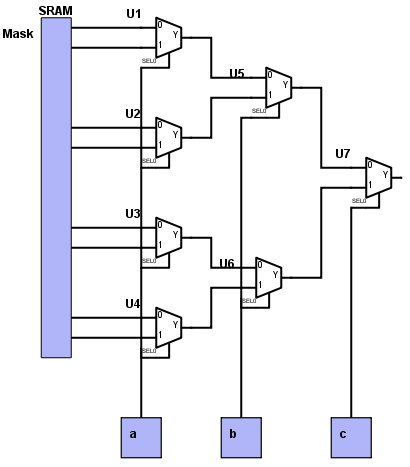
\includegraphics[height=.75\textheight,left]{lutMux.jpg}
\caption{$3$ stages of $2x1$ MUX}
\end{figure}

\column{.5\textwidth}
\begin{itemize}
\item It is a \alert{table} that ditermines what the output is for any given input
\item A \alert{state-less} interconnection of any number of gates \\(no feedback loops)
\item Implemented \emph{multiplexing} a combination of SRAM bits 
\end{itemize}


\end{columns}

\end{frame}
%------------------------------------------------

\begin{frame}
\frametitle{FPGAs Structure}
\framesubtitle{LUT Example}

$$y = ( a + b ) \cdot c $$

\begin{columns}[c]


\column{.4\textwidth}

\begin{table}
\centering
\begin{tabular}{c|c}
a b c & y \\
\hline
0 0 0 & 0\\
0 0 1 & 0\\
0 1 0 & 0\\
0 1 1 & 0\\
1 0 0 & 0\\
1 0 1 & 1\\
1 1 0 & 0\\
1 1 1 & 1\\

\end{tabular}
\end{table}

\column{.6\textwidth}
\centering
\begin{figure}
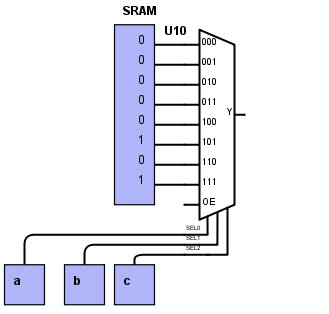
\includegraphics[width=.9\linewidth,left]{lutExplan.jpg}
\caption{$y = ( a + b ) \cdot c $ }
\end{figure}

\end{columns}
\end{frame}
%------------------------------------------------
\begin{frame}
\subsection{Basic Logic Element}
\frametitle{FPGAs structure}
\framesubtitle{BLE}

\begin{figure}
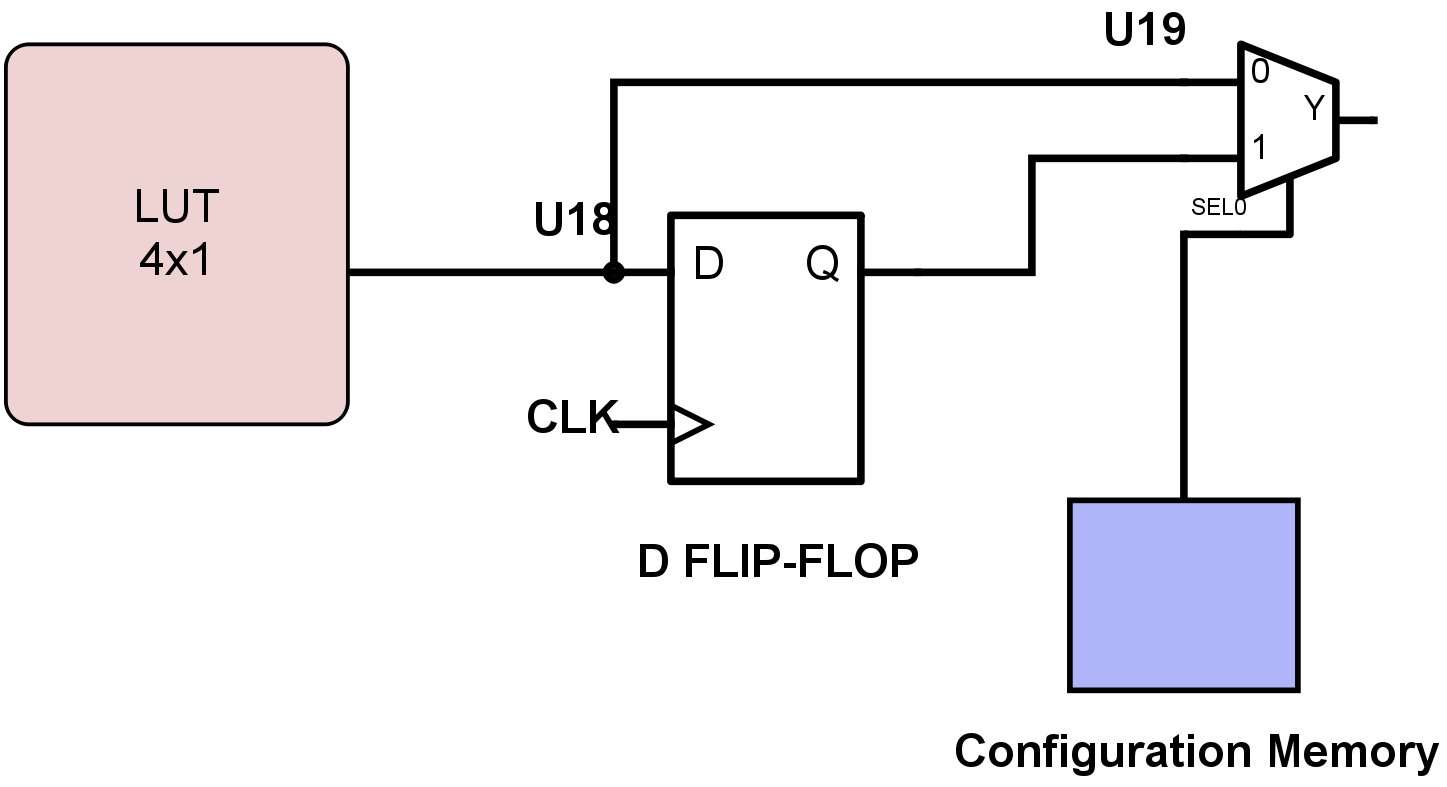
\includegraphics[width=.9\linewidth,left]{lutBLE.jpg}
\caption{Basic Logic Element}
\end{figure}

\end{frame}
%------------------------------------------------
\begin{frame}
\subsection{Overview}
\frametitle{FPGAs structure}
\framesubtitle{Overview}

\begin{figure}
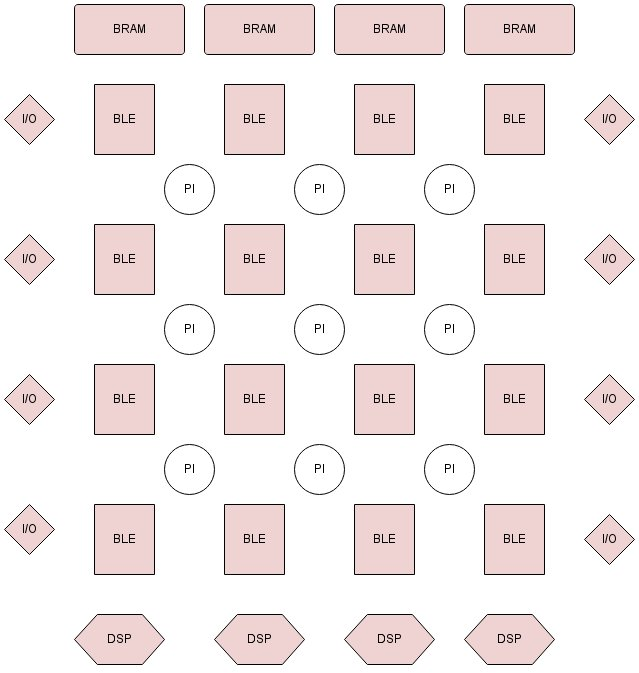
\includegraphics[width=.58\linewidth,center]{full.jpg}
\caption{FPGAs Complete Overview}
\end{figure}

\end{frame}


%------------------------------------------------
\begin{frame}
\section{Optimization Using HLS tools}
\subsection{Problem Description}
\frametitle{Problem Description}
\framesubtitle{Matrix Multiplication}


$$ C = A * B $$
$$c_{ij}=\sum_{k=1}^{n}a_{ik} \* b_{kj} $$

\begin{columns}[c]

\column{.01\textwidth}

\column{.3\textwidth}

\begin{tabular}{|c c c|}
$c_{11}$&\dots&$c_{1n}$\\
\vdots&\alert{$c_{km}$}&\vdots\\
$c_{n1}$&\dots&$c_{nn}$\\
\end{tabular}

\column{.4\textwidth}
\begin{tabular}{|c c c c|}
$a_{11}$&$a_{12}$&\dots&$a_{1n}$\\
\vdots&\vdots&&\vdots\\
\alert{$a_{k1}$}&\alert{$a_{k2}$}&\dots&\alert{$a_{kn}$}\\
\vdots&\vdots&&\vdots\\
$a_{n1}$&$a_{n2}$&\dots&$a_{nn}$\\
\end{tabular}

\column{.4\textwidth}
\begin{tabular}{|c c c c c|}
$b_{11}$&\dots&\alert{$b_{1m}$}&\dots&$b_{1n}$\\
$b_{21}$&\dots&\alert{$b_{2m}$}&\dots&$b_{2n}$\\
\vdots&&\vdots&&\vdots\\
$b_{n1}$&\dots&\alert{$b_{nm}$}&\dots&$b_{nn}$\\
\end{tabular}

\column{.2\textwidth}


\end{columns}


\end{frame}
%------------------------------------------------
\begin{frame}
\subsection{Serial Version}
\frametitle{No Directives}
$$c_{ij}=\sum_{k=1}^{n}a_{ik} \* b_{kj} $$
$$c_{km}=a_{k1}b_{1m}+a_{k2}b_{2m}+\dots+a_{kn}b_{nm}$$


\begin{columns}[c]
\column{.1\textwidth}
\column{.4\textwidth}

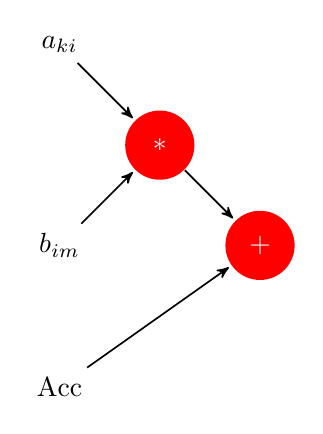
\begin{tikzpicture}[->,>=stealth',shorten >=1pt,auto,node distance=1.8cm, semithick]
  \tikzstyle{every state}=[fill=red,draw=none,text=white]

  \node[] (A) {$a_{ki}$};
  \node[state] (C) [below right of=A] {$*$};
  \node[] (B) [below left of=C] {$b_{im}$};
  \node[state] (D) [below right of=C] {$+$};
  \node[] (F) [below of=B]{Acc};
  
  \path (A) edge (C)
	(B) edge (C)
	(C) edge (D)
	(F) edge (D);
\end{tikzpicture}
\column{5\textwidth}

\begin{itemize}
\item $2n$ operations $\forall$ element
\item $n^2$ elements
\item[$\Rightarrow$] $2n^3$ operations
\item $19$MFLOPS on the tested platform
\end{itemize}


\end{columns}


\end{frame}

%------------------------------------------------
\begin{frame}
\subsection{Opt1: Inner Loop Unrolling}
\frametitle{Inner Loop Unrolling}
\framesubtitle{Opt1: Sum Mul Overlaping}


Our reference time interval is defined by the slowest operation which is the multiplication.

\begin{columns}[c]

\column{.3\textwidth}
\scalebox{0.8}{
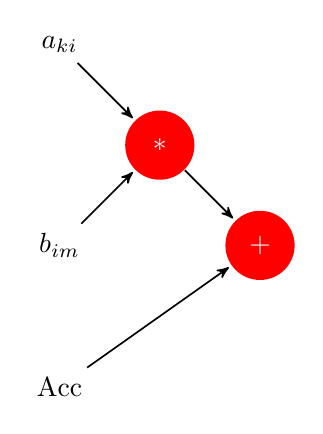
\begin{tikzpicture}[->,>=stealth',shorten >=1pt,auto,node distance=1.8cm, semithick]
  \tikzstyle{every state}=[fill=red,draw=none,text=white]

  \node[] (A) {$a_{ki}$};
  \node[state] (C) [below right of=A] {$*$};
  \node[] (B) [below left of=C] {$b_{im}$};
  \node[state] (D) [below right of=C] {$+$};
  \node[] (F) [below of=B]{Acc};
  
  \path (A) edge (C)
	(B) edge (C)
	(C) edge (D)
	(F) edge (D);
\end{tikzpicture}
}
\column{.2\textwidth}
\scalebox{0.9}{
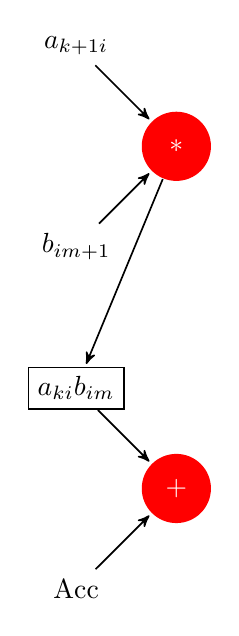
\begin{tikzpicture}[->,>=stealth',shorten >=1pt,auto,node distance=1.8cm, semithick]
  \tikzstyle{every state}=[fill=red,draw=none,text=white]

  \node[] (A) {$a_{k+1i}$};
  \node[state] (C) [below right of=A] {$*$};
  \node[] (B) [below left of=C] {$b_{im+1}$};
  \node[shape=rectangle,draw=black] (G) [below of=B] {$a_{ki}b_{im}$};
  \node[state] (D) [below right of=G] {$+$};
  \node[] (F) [below left of=D]{Acc};
  
  \path (A) edge (C)
	(B) edge (C)
	(C) edge (G)
	(G) edge (D)
	(F) edge (D);
\end{tikzpicture}
}
\column{.6\textwidth}
\begin{itemize}
\item Complete overlaping between Multiplication and addition
\item 35MFLOPS on the given machine
\end{itemize}

\end{columns}
\end{frame}
%------------------------------------------------
\begin{frame}
\subsection{Pipeline}
\frametitle{Pipeline}
\alert{Initiation Interval} is called the number of cycles between two new iterations.\\
In this case it is indicated by the time that the addition register is occupied.

\begin{columns}[c]
\column{.2\textwidth}
\scalebox{0.8}{
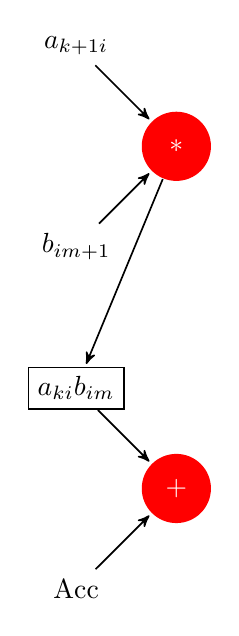
\begin{tikzpicture}[->,>=stealth',shorten >=1pt,auto,node distance=1.8cm, semithick]
  \tikzstyle{every state}=[fill=red,draw=none,text=white]

  \node[] (A) {$a_{k+1i}$};
  \node[state] (C) [below right of=A] {$*$};
  \node[] (B) [below left of=C] {$b_{im+1}$};
  \node[shape=rectangle,draw=black] (G) [below of=B] {$a_{ki}b_{im}$};
  \node[state] (D) [below right of=G] {$+$};
  \node[] (F) [below left of=D]{Acc};
  
  \path (A) edge (C)
	(B) edge (C)
	(C) edge (G)
	(G) edge (D)
	(F) edge (D);
\end{tikzpicture}
}
\column{.2\textwidth}
\scalebox{0.8}{
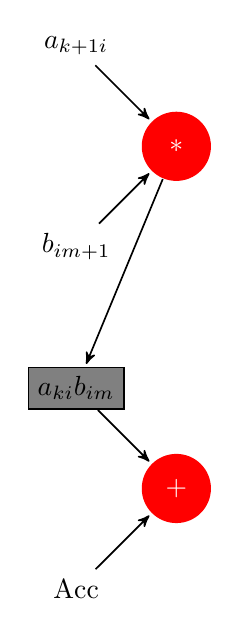
\begin{tikzpicture}[->,>=stealth',shorten >=1pt,auto,node distance=1.8cm, semithick]
  \tikzstyle{every state}=[fill=red,draw=none,text=white]

  \node[] (A) {$a_{k+1i}$};
  \node[state] (C) [below right of=A] {$*$};
  \node[] (B) [below left of=C] {$b_{im+1}$};
  \node[shape=rectangle,draw=black,fill=black!50] (G) [below of=B] {$a_{ki}b_{im}$};
  \node[state] (D) [below right of=G] {$+$};
  \node[] (F) [below left of=D]{Acc};
  
  \path (A) edge (C)
	(B) edge (C)
	(C) edge (G)
	(G) edge (D)
	(F) edge (D);
\end{tikzpicture}
}

\column{.5\textwidth}
\begin{figure}
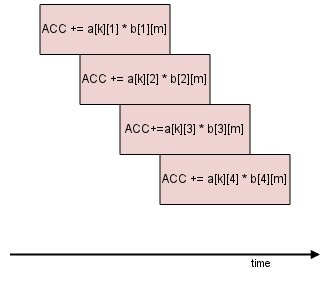
\includegraphics[width=.9\linewidth,center]{pipeline.jpg}
\end{figure}
\end{columns}
\end{frame}
%------------------------------------------------
\begin{frame}
\frametitle{J-loop unrolling}
\subsection{J-loop Unrolling}

\begin{columns}[c]

\column{.4\textwidth}
\begin{tabular}{c c c c}
\rowcolor{olive!15}
$a_{k1}$&$a_{k2}$&\dots&$a_{kn}$\\
\end{tabular}

\begin{beamercolorbox}[shadow=false,rounded=true]{box2}
{\usebeamercolor[fg]{text2} }
\begin{tabular}{c}
\\
\end{tabular}
\end{beamercolorbox}

\scalebox{0.8}{
\begin{beamercolorbox}[shadow=false,rounded=true]{box2}
{\usebeamercolor[fg]{text2} }
\begin{itemize}
\item Extra Hardware
\item Real Parallelism (Superscalar CPU architectures)
\item Expected scaling: $\times n$
\item Actual scaling: $\times 2$
\end{itemize}
\end{beamercolorbox}
}

\column{.1\textwidth}
\begin{table}
\begin{tabular}{ >{\columncolor{red!15}}c}
$b_{11}$\\
$b_{21}$\\
\vdots\\
$b_{n1}$\\
\end{tabular}
\end{table}
\scalebox{0.4}{
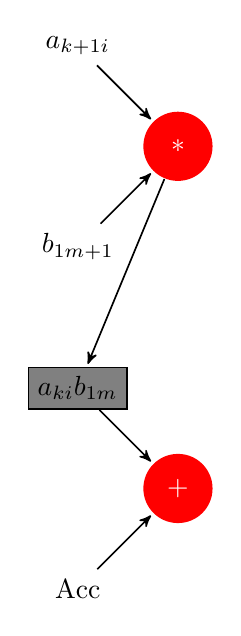
\begin{tikzpicture}[->,>=stealth',shorten >=1pt,auto,node distance=1.8cm, semithick]
  \tikzstyle{every state}=[fill=red,draw=none,text=white]

  \node[] (A) {$a_{k+1i}$};
  \node[state] (C) [below right of=A] {$*$};
  \node[] (B) [below left of=C] {$b_{1m+1}$};
  \node[shape=rectangle,draw=black,fill=black!50] (G) [below of=B] {$a_{ki}b_{1m}$};
  \node[state] (D) [below right of=G] {$+$};
  \node[] (F) [below left of=D]{Acc};
  
  \path (A) edge (C)
	(B) edge (C)
	(C) edge (G)
	(G) edge (D)
	(F) edge (D);
\end{tikzpicture}
}


\column{.1\textwidth}
\begin{table}
\begin{tabular}{ >{\columncolor{blue!15}}c}
$b_{12}$\\
$b_{22}$\\
\vdots\\
$b_{n2}$\\
\end{tabular}
\end{table}
\scalebox{0.4}{
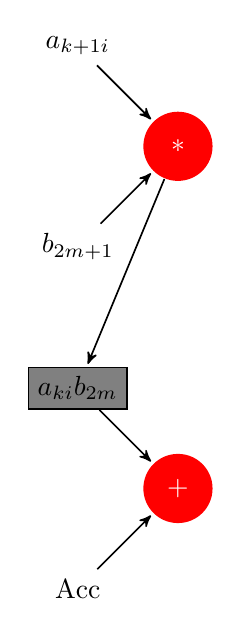
\begin{tikzpicture}[->,>=stealth',shorten >=1pt,auto,node distance=1.8cm, semithick]
  \tikzstyle{every state}=[fill=red,draw=none,text=white]

  \node[] (A) {$a_{k+1i}$};
  \node[state] (C) [below right of=A] {$*$};
  \node[] (B) [below left of=C] {$b_{2m+1}$};
  \node[shape=rectangle,draw=black,fill=black!50] (G) [below of=B] {$a_{ki}b_{2m}$};
  \node[state] (D) [below right of=G] {$+$};
  \node[] (F) [below left of=D]{Acc};
  
  \path (A) edge (C)
	(B) edge (C)
	(C) edge (G)
	(G) edge (D)
	(F) edge (D);
\end{tikzpicture}
}

\column{.1\textwidth}
\begin{tabular}{c}
\dots\\
\dots\\
\\
\dots\\
\end{tabular}

\begin{beamercolorbox}[shadow=false,rounded=true]{box2}
{\usebeamercolor[fg]{text2} }
\begin{tabular}{c}
\\\\\\\dots\\\\\\\\
\end{tabular}
\end{beamercolorbox}

\column{.1\textwidth}
\begin{table}
\begin{tabular}{ >{\columncolor{green!15}}c}
$b_{1n}$\\
$b_{2n}$\\
\vdots\\
$b_{nn}$\\
\end{tabular}
\end{table}
\scalebox{0.4}{
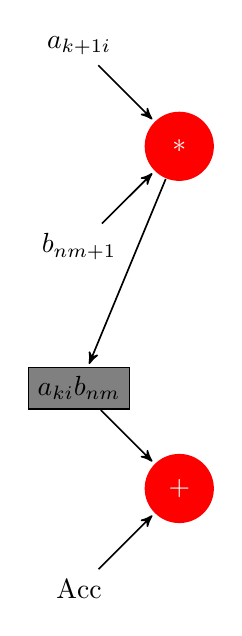
\begin{tikzpicture}[->,>=stealth',shorten >=1pt,auto,node distance=1.8cm, semithick]
  \tikzstyle{every state}=[fill=red,draw=none,text=white]

  \node[] (A) {$a_{k+1i}$};
  \node[state] (C) [below right of=A] {$*$};
  \node[] (B) [below left of=C] {$b_{nm+1}$};
  \node[shape=rectangle,draw=black,fill=black!50] (G) [below of=B] {$a_{ki}b_{nm}$};
  \node[state] (D) [below right of=G] {$+$};
  \node[] (F) [below left of=D]{Acc};
  
  \path (A) edge (C)
	(B) edge (C)
	(C) edge (G)
	(G) edge (D)
	(F) edge (D);
\end{tikzpicture}
}


\end{columns}

\alert{Memmory Bounds}: Dual Channeled memory $\implies$ only $2$ concurent operations.
\end{frame}
%------------------------------------------------
\begin{frame}
\subsection{Array Partitioning}
\frametitle{Row / Col Partitioning}

\begin{columns}[c]


\column{.5\textwidth}
\begin{figure}
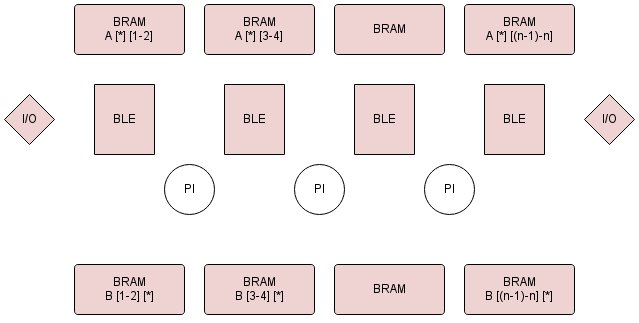
\includegraphics[width=1.2\linewidth,center]{arraysplit.jpg}
\caption{Distribute the array into multiple BRAMS}
\end{figure}

\column{.5\textwidth}

\end{columns}

\end{frame}
%------------------------------------------------
\begin{frame}
\subsection{}
\frametitle{}

\end{frame}
%------------------------------------------------
%------------------------------------------------
%------------------------------------------------
%------------------------------------------------
%------------------------------------------------


\end{document} 
%----------------------------------------------------------------------------------------
